\documentclass[
	11pt,								% 11 Punkt Schrift verwenden (auch 10pt, 12pt moeglich)
	a4paper,						% Dokumentgroesse A4
	oneside,						% einseitiger Druck (auch twoside moeglich)
	titlepage,					% Titelblatt generieren
	headsepline,				% Kopfzeile duch Linie vom text getrennt
	DIV13,							% Groesse des Satzspiegels
	abstracton,	 				% zeigt die Abstractueberschrift (abstracton oder abtractoff)
	BCOR0cm,						% Groesse des Bindungsrandes (z. B.: BCOR2.5cm)
	bibliography=totoc, % bibliography is added to the table of contents
]{scrreprt}							% Dokumentenklasse (KomaScript - Report)
%]{report}							% Dokumentenklasse (Native Latex - Report)

% MATH, FORMULAE AND SIGNS PACKAGES
\usepackage{amsmath}								% besser als standard math
\usepackage{amssymb}

% LANGUAGE PACKAGES
%\usepackage[german]{				% Anpassungen ensprechend der Sprache
%\usepackage[latin1]{inputenc}
\usepackage[ngerman]{babel}
\usepackage[T1]{fontenc}

\usepackage[utf8]{inputenc}				% direkte Eingabe von Umlauten
\usepackage{csquotes}							% Anfuehrungszeichen entsprechend der Sprache

% GRAPHIC PACKAGES
\usepackage{graphicx}							 % Packet zu Einbindung von Graphiken
\usepackage{subfig}									% fuer die Erstellung von Unterabbildungen
\usepackage{wrapfig}

% LAYOUT PACKAGES
\usepackage{fancyhdr}
\usepackage{parskip}								% besseres Absatzlayout (Leerzeile statt Einrückung)
\usepackage[official,right]{eurosym}% für ein \euro{} Symbol
\usepackage{hyperref}							% F\"ur Hyperlinks
\hypersetup{
	hypertexnames=true,
	unicode = {true},
	colorlinks = {true},
	pdftitle = {Entwicklung eines Systems ...},
	pdfauthor = {Christian Schaub},
	pdfkeywords = {keywords},
	pdfborder = {0 0 0},
	linkcolor = black,
	citecolor = black,
	urlcolor = black,
	breaklinks = true,
}
\usepackage{url}										% fuer URLs als Literaturverzeichnis
\usepackage{color}
\usepackage{setspace}
\usepackage{rotfloat}
%\usepackage{verbatim}								% multiline comments
\usepackage{nextpage}
\usepackage[textsize=scriptsize]{todonotes}
\usepackage[numbers]{natbib}


%\usepackage[
%	block=nbpar,
%	citestyle=numeric-comp,
%	bibstyle=stopfer,
%	maxbibnames=10
%]{biblatex}
%\addbibresource{bibtex_database.bib}

% OPTIONS, DEFINITIONS
\usetikzlibrary{arrows,automata,shapes.multipart,trees}
\onehalfspacing							% anderthalbzeilig (oder auch \doublespace)
\pagestyle{headings}				% Überschrift in der Kopfzeile und Seitenzahlen
\setcapindent{0mm}
\addtokomafont{caption}{\small}

% OWN COMMANDS

% Adding lines above and below the chapter head
\newcommand*{\ORIGchapterheadstartvskip}{}
\let\ORIGchapterheadstartvskip=\chapterheadstartvskip
\renewcommand*{\chapterheadstartvskip}{
	 \ORIGchapterheadstartvskip{
			 \setlength{\parskip}{-40pt}
			 \noindent\rule{.3\textwidth}{3pt}\rule[2.5pt]{.7\linewidth}{.5pt}\par
	 }
}

\newcommand*{\ORIGchapterheadendvskip}{}
\let\ORIGchapterheadendvskip=\chapterheadendvskip
\renewcommand*{\chapterheadendvskip}{
	 {
			 \setlength{\parskip}{0pt}
			 \noindent\rule{.3\textwidth}{.5pt}\par
	 }
	 \ORIGchapterheadendvskip
}

\newcommand{\eclipse}{$\mbox{ECL}^i\mbox{PS}^e$}

%%%%%%%%%%%%%%%%%%%%%%%%%%%%%%%%%%%DOCUMENT%%%%%%%%%%%%%%%%%%%%%%%%%%%%%%%%%%%%%

\begin{document}

% Cover
	%\pagenumbering{alpha}
	\thispagestyle{empty}
	
\includegraphics[height=1.2cm]{images/vsLogo.png}
	\hfill
\includegraphics[height=1.2cm]{images/uniLogo.pdf}\\[1cm]

	\begin{center}
		\begin{LARGE}\bfseries Reaktives Hardwaremonitoring autonomer Roboter \end{LARGE}\\
		%, oder : Hardwaremonitoring autonomer mobiler Roboter durch reaktive Agenten oder : Reaktive Agenten zur Überwachung der Hardware eines autonomen mobilen Roboters
		[2cm]
		\Large{Universität Kassel}\\
		[1cm]
		\large{Projektbericht von}\\
		\Large{Christian Schaub}\\
		[1cm]
		\large \Large{Fachgebiet Verteilte Systeme \\
		Universität Kassel}\\
		[1cm]
	\end{center}
	
%	\begin{abstract}
%	Kurze Beschreibung des Projektes
%	\end{abstract}


	\vfill
	\begin{Large}
		\begin{tabular}{l l}
			Gutachter: & Prof. Dr. Kurt Geihs\\
			[1cm]
			Betreuer: & Dipl.-Ing. Dominik Kirchner\\
		\end{tabular}
	\end{Large}
	\vfill2

	\begin{center}Datum: Januar 21, 2013\end{center}

	

	\tableofcontents

	
	%% Hier können die einzelnen Kapitel inkludiert werden. Sie müssen in den 
% entsprechenden .TEX-Dateien vorliegen. Die Dateinamen können natürlich 
% angepasst werden.
%\include{Inhalt/Akronyme} %Akronyme.tex
\chapter{Related Work}
\label{cha:Related Work}

\section{Section 2}
\label{sec:2Section2}
Willkommen im Portal f"ur Elektronik, Maschinenbau und Mechatronik !
Dieses Portal soll euch beim lernen und diskutieren der einzelnen Studienf"acher behilflich sein, oder im Alltag als Knowledge-Base zur Verf"ugung stehen ! \\
F"ur jedes Studienfach wird in einem "Ubersichtsartikel der Inhalt zusammengefasst und die einzelnen Fachartikel in Beziehung zueinader gestellt. 
Kommen Formeln in den Fachartikeln vor, werden diese in einer Formelsammlung zu dem jeweiligen Studienfach zusammengef"uhrt. 
Am Ende soll jedes Studienfach eine"Ubersichtsartikel und wenn m"oglich eine Formelsammlung besitzen.

\subsection{Subcestion 2.1}
\label{subsec:2Subcestion2.1}

\begin{figure}[htb]
\centering
\includegraphics[width=0.2\textwidth]{mkDoc-Logo.png}
\caption{mkDoc}
\label{fig:mkDoc}
\end{figure}


\subsection{Subcestion 2.2}
\label{subsec:2Subcestion 2.2}
Willkommen im Portal f"ur Elektronik, Maschinenbau und Mechatronik !\footnote{\Vgl\Zitat[S.~11]{Sicherheitstechnik}}
Dieses Portal soll euch beim lernen und diskutieren der einzelnen Studienf"acher behilflich sein, oder im Alltag als Knowledge-Base zur Verf"ugung stehen ! \\
F"ur jedes Studienfach wird in einem "Ubersichtsartikel der Inhalt zusammengefasst und die einzelnen Fachartikel in Beziehung zueinader gestellt. 
Kommen Formeln in den Fachartikeln vor, werden diese in einer Formelsammlung zu dem jeweiligen Studienfach zusammengef"uhrt. 
Am Ende soll jedes Studienfach einen  "Ubersichtsartikel und wenn m"oglich eine Formelsammlung besitzen.

 %Einleitung.tex
\include{Inhalt/Relatedwork} %Vorgaben.tex
\include{Inhalt/Konzept} %Entwicklung.tex
\include{Inhalt/Umsetzung} %Umsetzung.tex
\include{Inhalt/Evaluierung} %Fazit.tex
\include{Inhalt/Zusammenfassung} %Zusammenfassung.tex

 %Inhalt.tex
\chapter{Einleitung}
\label{cha:Einleitung}


Das Forschungsgebiet autonome Robotik steht aufgrund der durch die Roboter autonom entschiedenen Aktionen neuen Herausforderungen, die Zuverlässigkeit\footnote
{Wahrscheinlichkeit einer fehlerfreien Anwendung über eine spezifizierte Zeitdauer\cite{3}}
der entwickelten Roboter betreffend, gegenüber\cite{2}.
Autonome mobile Roboter bewegen sich frei in ihren jeweiligen Einsatzgebieten und müssen dadurch unter anderem in der Lage sein sich selbstständig in diesem Gebiet
zu orientieren. Im Gegensatz zu Robotern mit $statischen Routen$ festen Wegpunkten ist hier das Gefährdungspotenzial für den Benutzer und die Umgebung weitaus höher\cite{1}.
Als Beispiel können die Fußballroboter des Fachgebietes dienen\cite{4}. Diese können durch ihren Aufbau, das damit verbundene Gewicht von 30kg und ihrer
maximalen Geschwindigkeit von 4 m/s eine Gefahr darstellen.
Um die von diesem System ausgehenden Gefahren zu minimieren, ist eine verlässliche Sensorik und Aktorik notwendig um die Roboter selbst, sowie deren Nutzer und die Umgebung zu schützen.
Sämtliche Aktorik und Sensorik ist auf bestimmte physikalische Gegebenheiten angewiesen, um nach Spezifikation zu funktionieren. Viele Microcontroller benötigen beispielsweise eine bestimmte stabilisierte Betriebsspannung.\\
Im Rahmen dieses Projektes wurden daher Möglichkeiten untersucht unterschiedlichste relevante physikalische Größen
in einem autonomen Robotersystem zu erfassen, diese Daten für weitergehende Diagnosen zu kommunizieren und schnelle Reaktionen auf diese Daten 
Editieren
direkt auf der Controllerebene auszuführen. Ein Beispiel wäre hier die sofortige Deaktivierung eines Sensors, sollte eine Betriebsspannung außerhalb der Spezifikation anliegen.\\
Die grundsätzliche Verarbeitung und Auswertung der erfassten Daten findet weiterhin im Robotersystem selbst statt.
Um die Verfügbarkeit der erfassten Messwerte im Robotersystem sicherzustellen, werden diese redundant zum Robotersystem übermittelt.\\
Auf die einzelnen Schritte vom Formulieren der Problemstellung über konzeptionelle Entscheidungen bis zur Umsetzung und Evaluierung wird in den folgenden Kapiteln eingegangen.\\


Related Work:
-


% ab Einleitung zählen !!
\pagenumbering{arabic}




\chapter{Problemstellung}
\label{cha:Problemstellung}
Autonome Roboter bestehen aus mechanischen und elektronischen Komponenten und sind, wie einleitend beschrieben, 
schnell und schwer genug um sich selbst, die Umgebung oder Personen zu gefährden. 
Ziel dieses Projektes ist ein Beitrag zur Steigerung der Zuverlässigkeit eines autonomen Roboters. Hierzu soll im Rahmen des vorgestellten
Projektes eine Überwachung von systemrelevanten physikalischen Größen\footnote{elektrische Spannung, Temperatur, Licht \cite{5}},
deren Ausprägung Rückschlüsse über den Zustand wichtiger mechanischer oder elektronischer Komponenten zulassen können und die Möglichkeit einer Reaktion umgesetzt werden.\\
Um einerseits die erfassten Daten dem Robotersystem zur weiteren Auswertung übermitteln zu können und andererseits die Einstellung bestimmter Parameter, 
sowie die Steuerung der Aktionen des Meßsystems durch das Robotersystem zu ermöglichen, muß eine ausfallsichere Kommunikation zwischen dem Roboter- und Meßsystem
ermöglicht werden.\\
Durch die eingangs beschriebene Problemstellung ergeben sich mehrere zu lösende Aufgaben.
Zum einen müssen Möglichkeiten untersucht werden physikalische Größen, wie Spannungen, Temperaturen oder Licht zu messen.
Zum anderen soll das Meßsytem direkt entsprechende Reaktionen durchführen können, sollten die Meßwerte bestimmte Sicherheitskriterien verletzen. 
Zudem müssen die Daten zum Robotersystem übertragen werden, um weitere Auswertungen vornehmen zu können.\\
Um eine möglichst allgemeine Anwendbarkeit zu erreichen(z.B. große Systeme mit einer Vielzahl zu erfassender Meßgrößen), ist die Skalierbarkeit\footnote{Steigerung der Leistung(hier: Anzahl der erfassbaren Meßgrössen des Systems durch das Hinzufügen zusätzlicher Meßknoten)\cite{6}}
des Meßsystems durch eine dezentrale Organisation mehrerer paralleler Meßsysteme in einem Robotersystem vorzusehen.\\

Zusammenfassend ergeben sich folgende Grundfunktionalitäten des Meßsystems:
\begin{enumerate}
 \item Messen physikalischer Größen
 \item Kommunikation 
 \item Reaktionen durch das Meßsystem
\end{enumerate}



%\end{tabbing}



\chapter{Konzept}
\label{cha:Konzept}

Im folgenden Kapitel werden die Konzepte zum Bereitstellen der in Kapitel 2 diskutierten Grundfunktionalitäten des zu konzipierenden 
Systems dargestellt und der in Abbildung~\ref{fig:Grundfunktionaltäten} grundlegend dargestellte Entwurf des Meßsystems weiter konkretisiert.

\begin{figure}[htb]
\centering
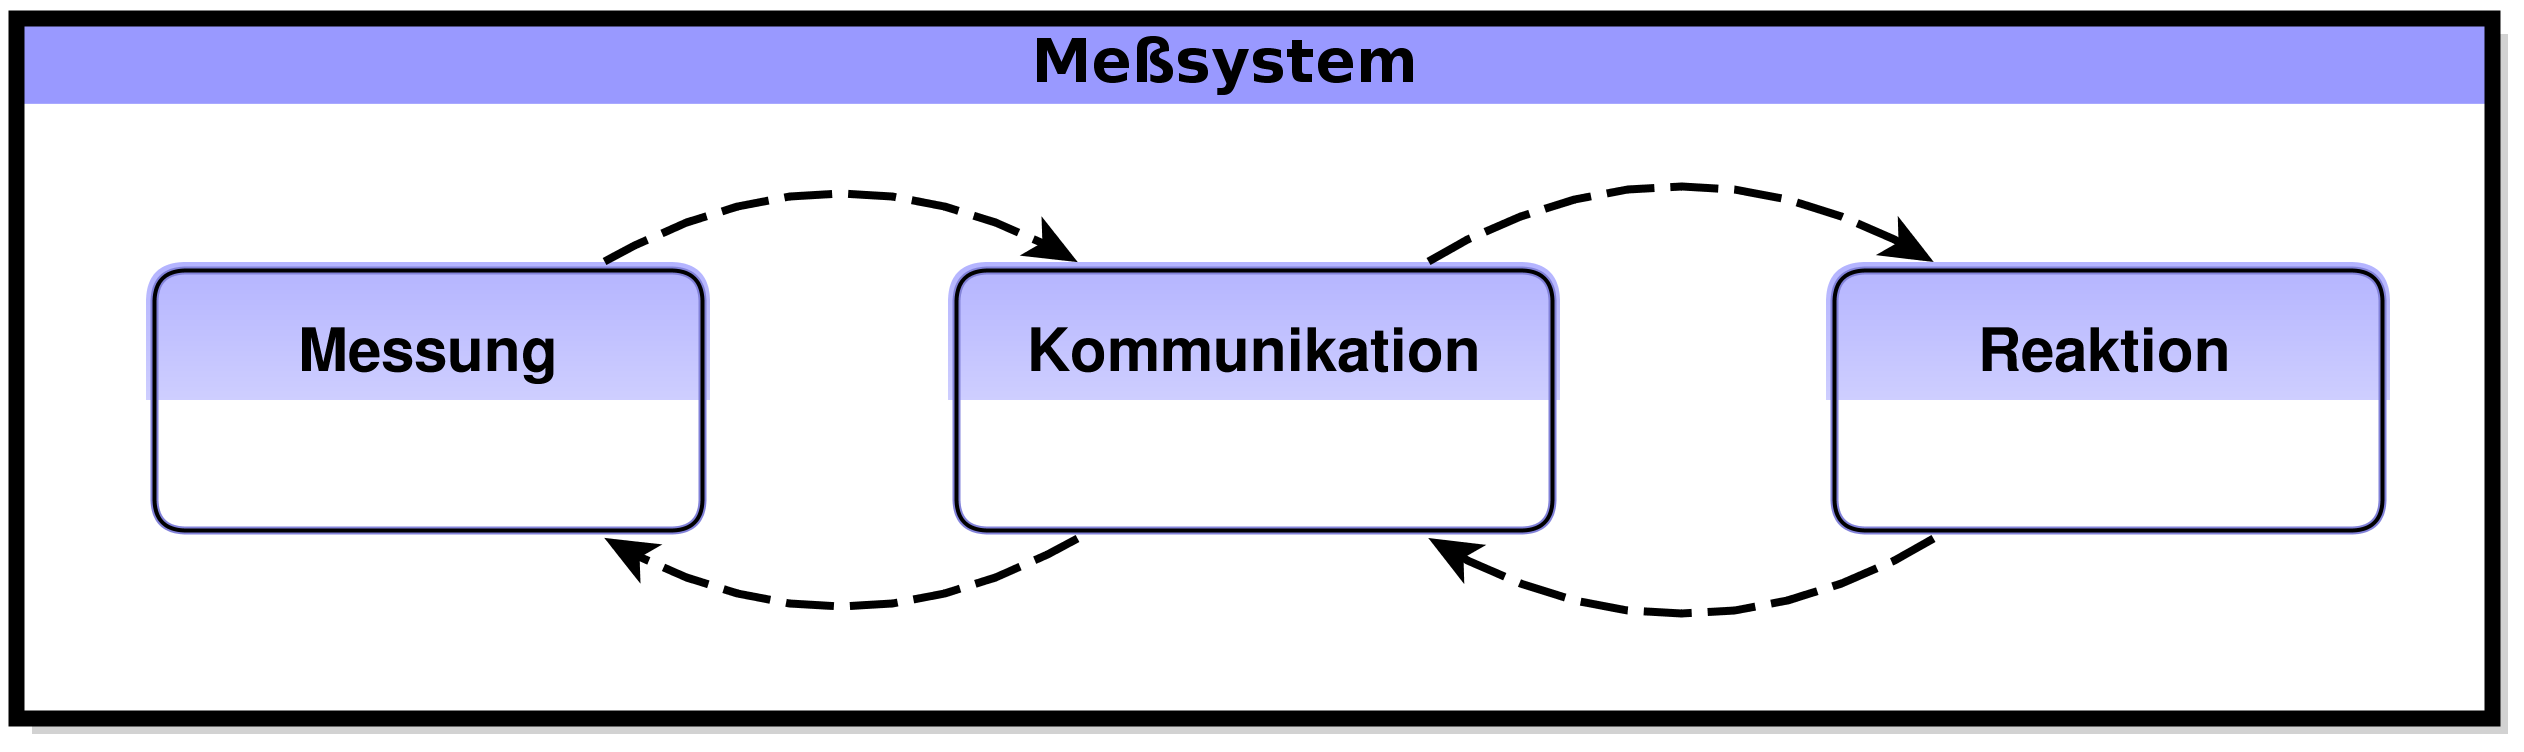
\includegraphics[width=0.6\textwidth]{images/schau1neu.png}
\caption{erster Entwurf des Meßsystems}
\label{fig:Grundfunktionaltäten}
\end{figure}
Ein reaktives Meßsystem setzt einerseits die Möglichkeit einer lokalen Informationserfassung- und verarbeitung voraus.
Andererseits muß jedes Meßsystem, auch auf Grund der nötigen dezentralen Organisation mehrerer paralleler Meßsysteme(Skalierbarkeit), selbstständig 
einfache Entscheidungen treffen können. Das Meßssystem benötigt demnach eine Kontrolleinheit, diese sollte in Lage sein eventuell durch 
das Ansteuern von Peripherie, die Kommunikation zum Robotersystem zu steuern und Befehle vom Robotersystem zu empfangen und auszuführen. Ein derartiges Meßsystem, 
Abbildung ~\ref{fig:schaubild2} zeigt den konkretisierten Aufbau, stellt einen lokalen reaktiven Agenten\cite{7} dar. 
\begin{figure}[htb]
\centering
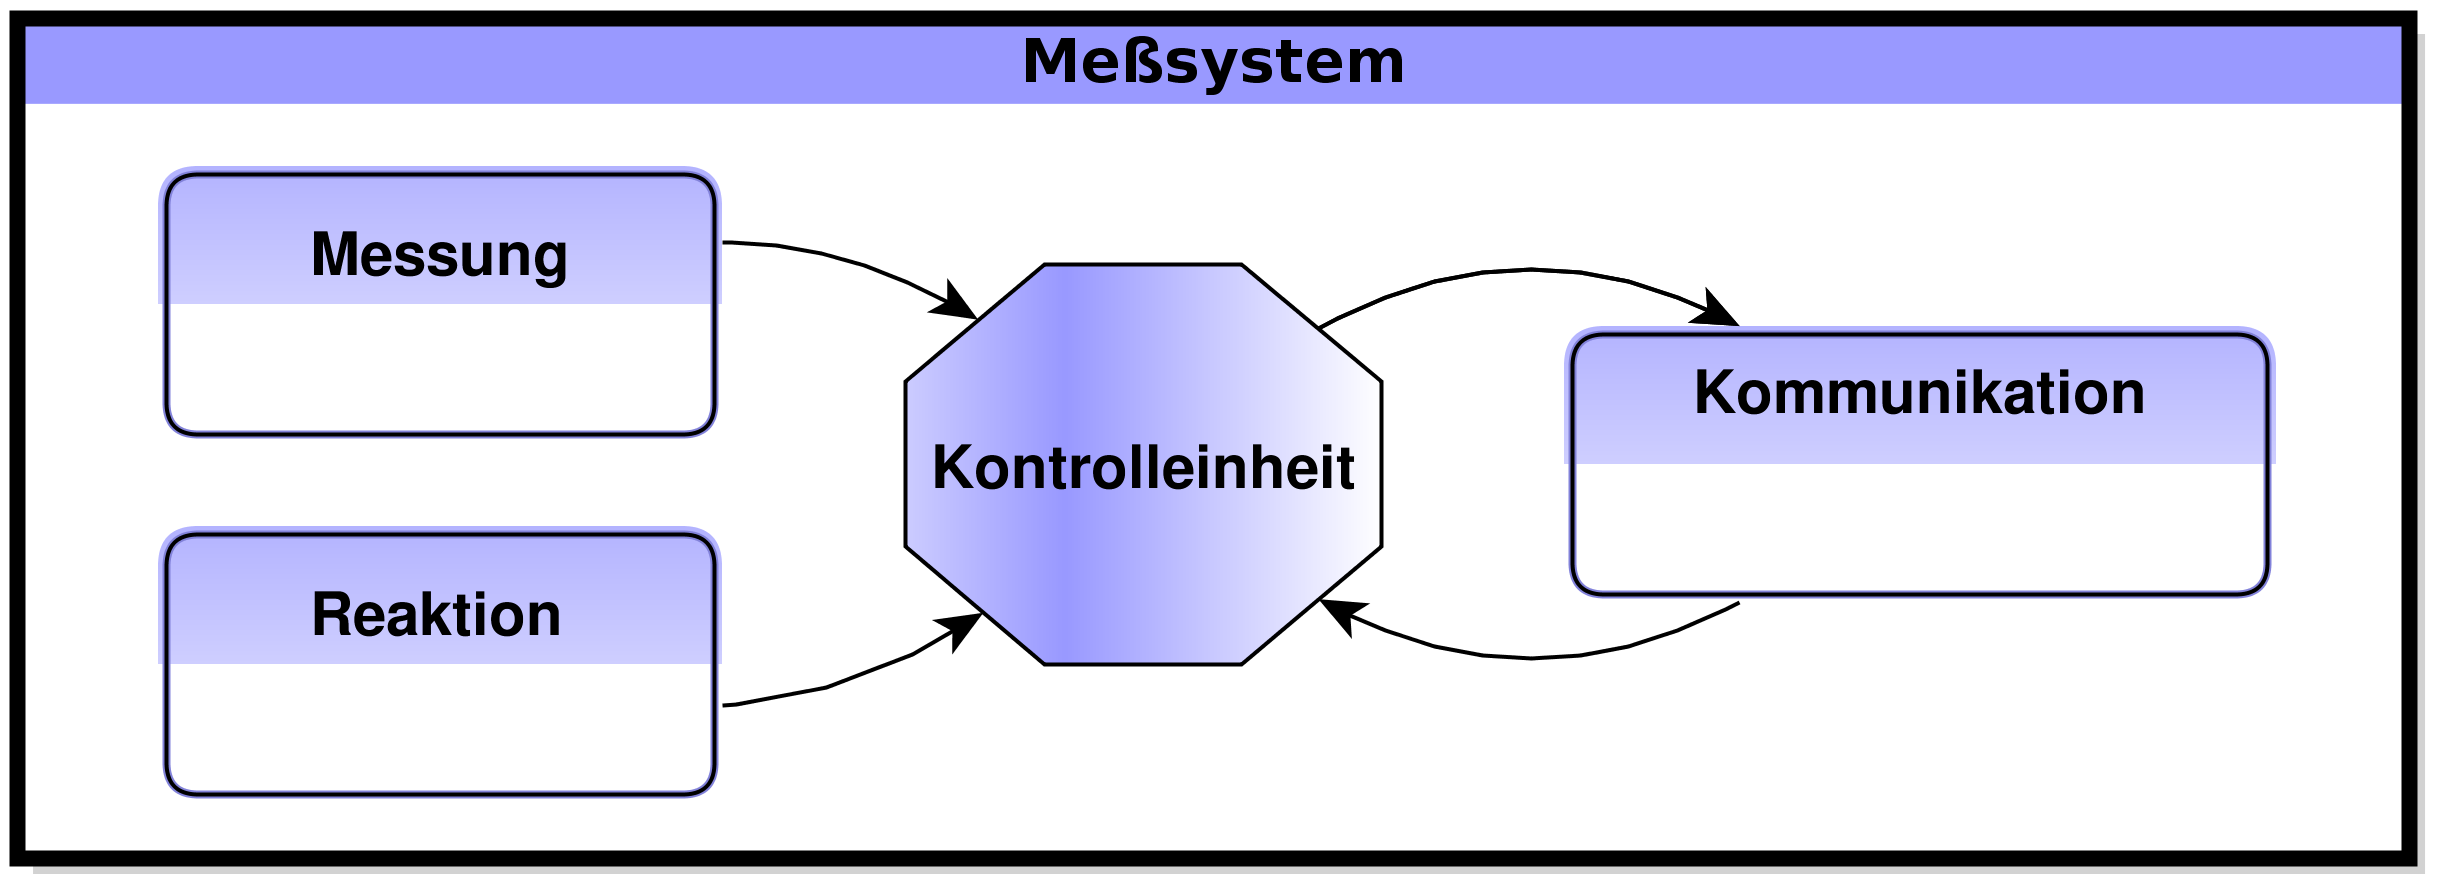
\includegraphics[width=0.6\textwidth]{images/schau2cool.png}
\caption{Meßsytem mit Kontrolleinheit}
\label{fig:schaubild2}
\end{figure}

Die angestrebten Funktionalitäten sind grundsätzlich unabhängig, daher werden die Konzepte zur Entwicklung der Funktionalitäten Messen, Kommunikation und 
Reaktion in den folgenden Unterkapiteln getrennt diskutiert.


%\begin{enumerate}
  \section{ Messen physikalischer Größen}
  Zur Spannungsmessung stehen sogenannte ADC\footnote{Analog-Digital-Converter} Eingänge, zum Konvertieren der analogen Messwerte in digitale Werte zur Verfügung.
  Das Messen anderer physikalischer Grössen erfolgt über Sensoren, diese geben Spannungswerte aus, die mittels des ADC in digitale Werte konvertiert werden. 
  Die erfassten digitalen Spannungswerte müssen zunächst durch eine Kontrolleinheit, mittels der im Datenblatt des Sensors festgelegten Formeln oder Tabellen ausgewertet und in die tatsächliche
  physikalische Größe umgerechnet werden. Zu beachten ist, daß die maximale Höhe der durch einen ADC erfassbaren Spannung durch die Höhe dessen Versorgungsspannung begrenzt wird. Sollen Spannungen 
  über der Versorgungsspannung des ADC erfasst werden, müssen diese vor der Messung durch den ADC mit geeigneten messtechnischen Verfahren auf die maximal zulässige Spannung reduziert werden. Die Umrechnung in den
  tatsächlichen Wert übernimmt anschließend die Kontrolleinheit, daher muß der Kontrolleinheit das Verhältnis bekannt sein, das die Reduzierung der zu messenden Spannung bestimmt. 

  \section{ Kommunikation}
  Die Kontrolleinheit sollte mehrere Kommunikationskanäle bereitstellen, um die Kommunikation zu angesteuerten Komponenten des Meßsystems selbst und dem Robotersystem zu ermöglichen.
  Um diese Kommunikation zu ermöglichen, sind verschiedene Bussysteme verfügbar, durch die Kontrolleinheit gesteuerte Komponenten des Meßsystems
  realisieren und steuern den Bus. Um eine ausfallsichere Übertragung der systemrelevanten Daten zu gewährleisten, sollte die Kommunikation redundant erfolgen.
  
  \section{ Reaktionen durch das Meßsystem}
  Reaktionen durch das Meßsystem erfordern einerseits die Möglichkeit einer einfachen Zweipunktregelung\footnote{Regler mit zwei Ausgangszuständen. Je nachdem, ob der Istwert über oder unter dem Sollwert liegt, wird der obere oder der untere Ausgangszustand eingenommen. Quelle:http://de.wikipedia.org/wiki/Zweipunktregler} der überwachten Komponenten durch das Meßsystem und andererseits die eingangs beschriebene
  Möglichkeit einfache Entscheidungen durch eine Kontrolleinheit lokal zu treffen und Befehle des Robotersystems auszuführen. Sollen Komponenten überwacht werden, deren Betriebsstrom zu hoch ist um diese direkt zu regeln,
  muß es durch geeignete Verfahren der Meß- und Regelungstechnik ermöglicht werden diese Komponenten indirekt zu regeln. Die Kontrolleinheit steuert in diesem Fall diese Regelung.
%\end{enumerate}

Um ein generisch einsetzbares Meßsystem zu konstruieren, muß es möglich sein unterschiedliche Meßbereiche zu erfassen. Daher sind konfigurierbare Meßbereiche und 
ein dementsprechend modularer Aufbau der Meßvorrichtung des Meßsystems vorzusehen.

Zusammenfassend ergibt sich folgendes Konzept, wie durch Abbildung ~\ref{fig:schaubild2} dargestellt:

\begin{itemize}
 \item Lokale Reaktivität durch on-board Verarbeitung der Messwerte.
 
\item Generischer Einsatz durch Nutzung der Trennung von Sensorik und ADC durch modulares Design der Meßvorrichtung.

\item Skalierbarkeit durch dezentrales Design und redundante(Ausfallsicherheit) Kommunikation.
\end{itemize}

\begin{figure}[htb]
\centering
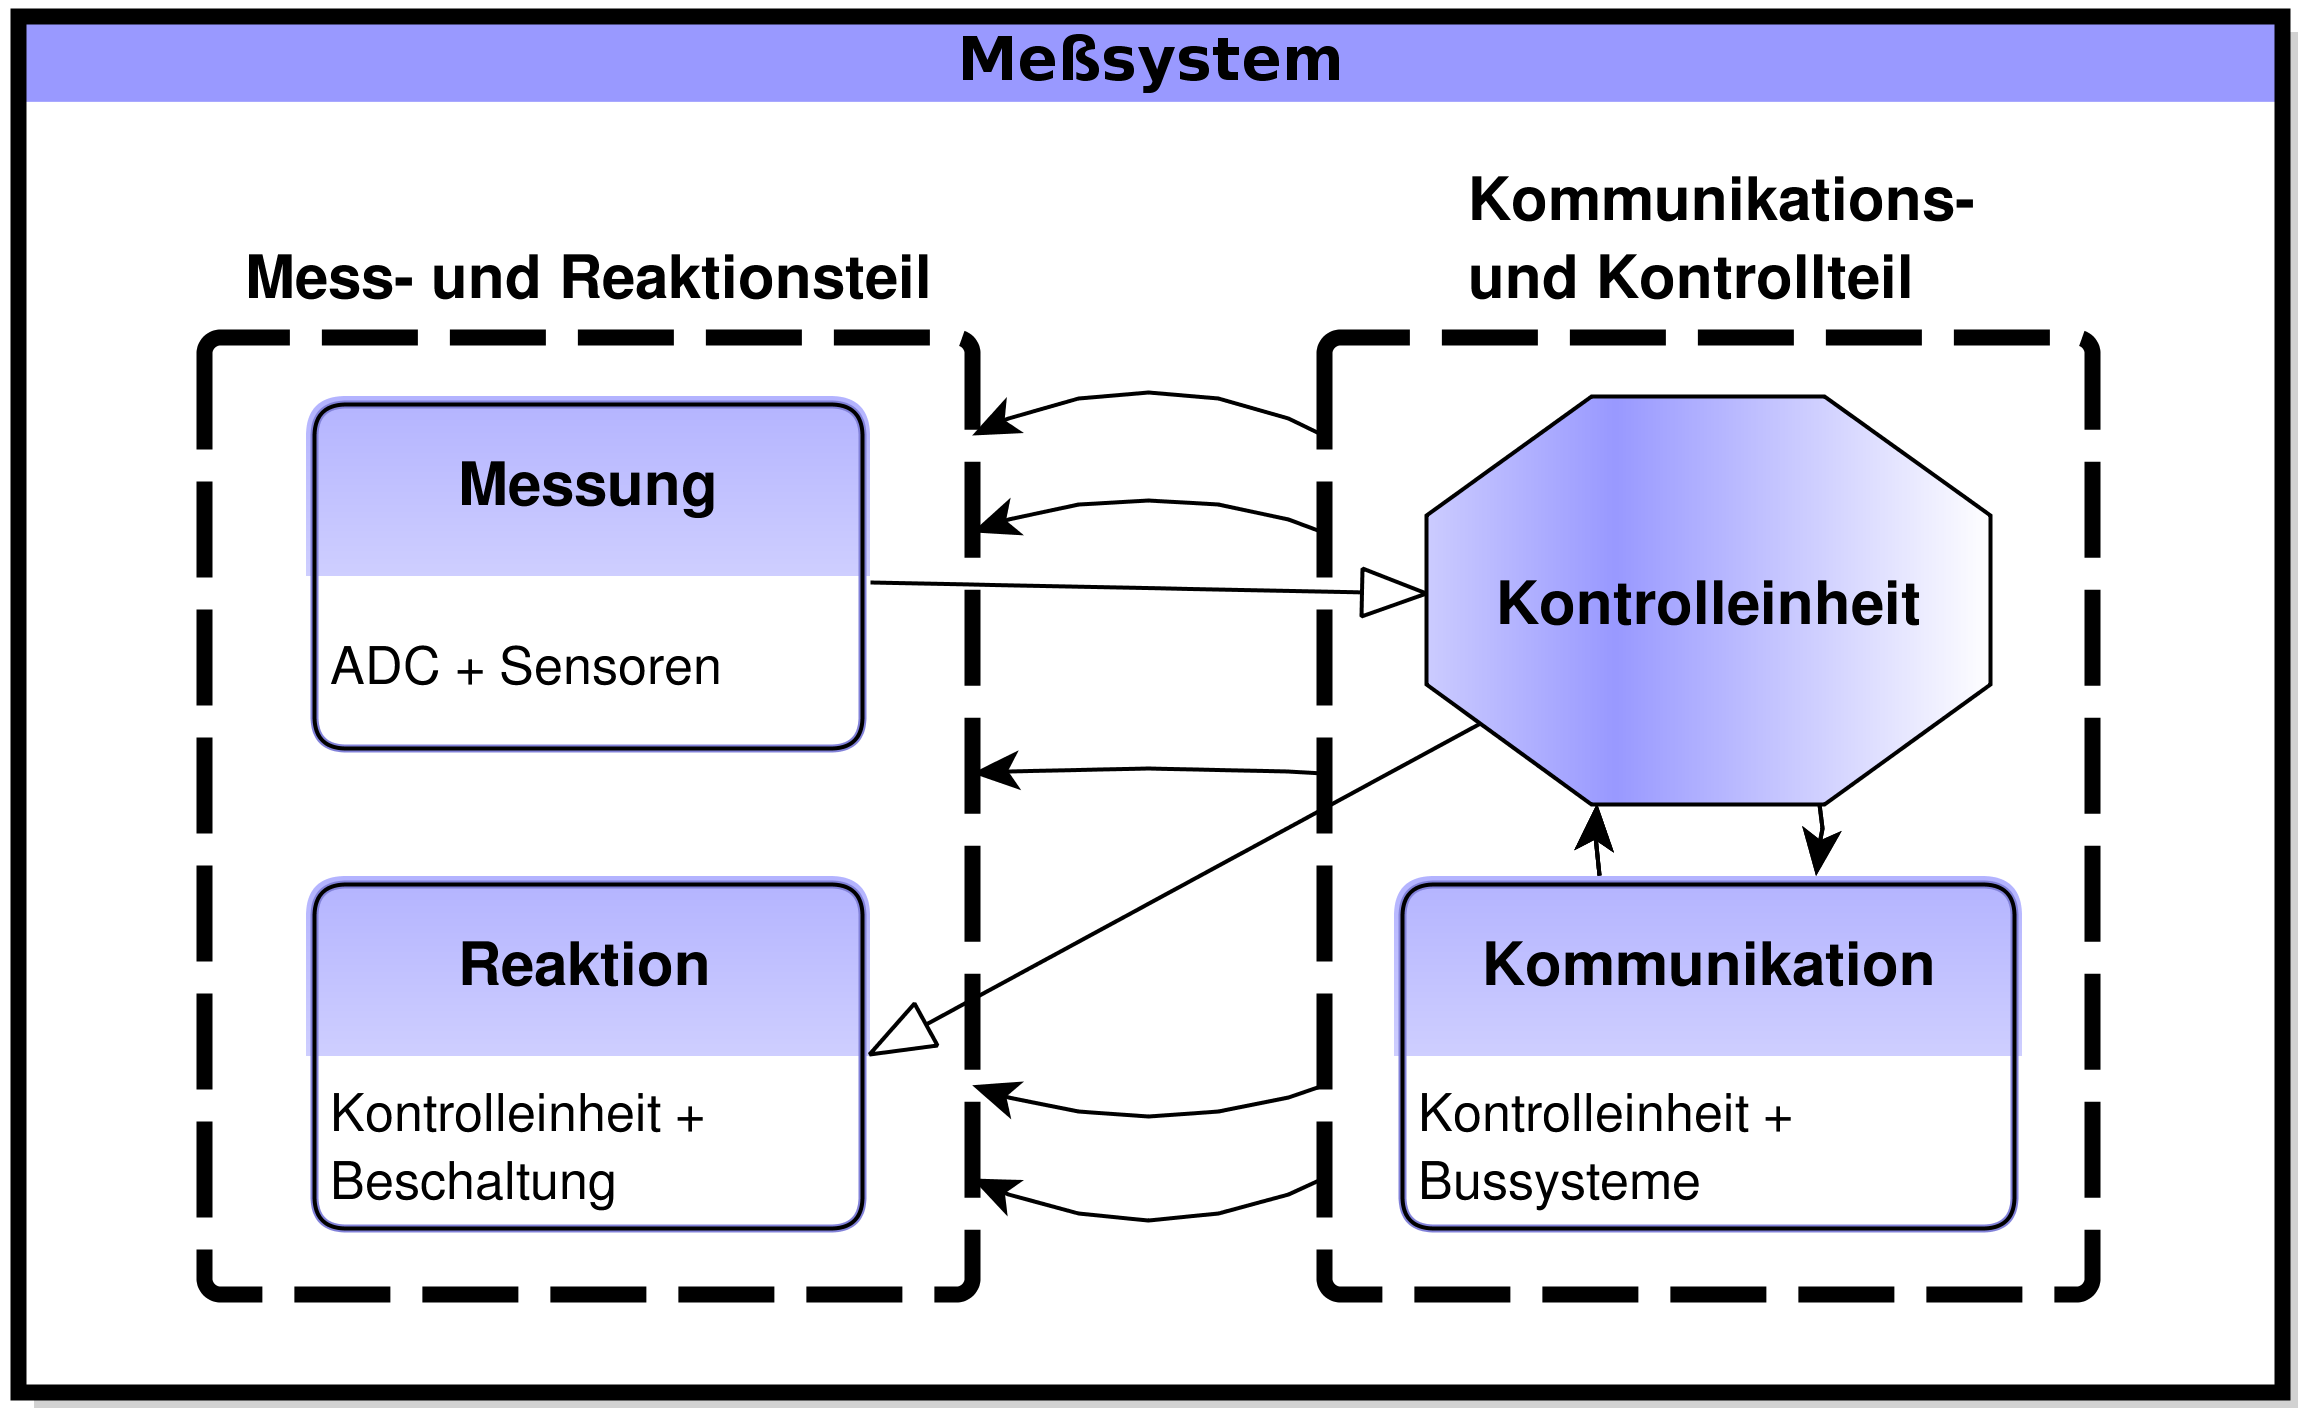
\includegraphics[width=0.6\textwidth]{images/schau3cool.png}
\caption{Meßsytem mit modularem Meßteil und Kontrolleinheit}
\label{fig:schaubild2}
\end{figure}



\chapter{Umsetzung}
\label{cha:Umsetzung}
In diesem Kapitel, wird die Umsetzung zuvor dargestellten Konzeptes beschrieben. Zunächst wird die 
Umsetzung der Hardwarekomponenten beschrieben, anschließend folgt die Beschreibung der Software des Microcontrollers und des Robotersystemes.
\section{Hardware}
Die konzeptionell als Kontrolleinheit bezeichnete Komponente des Systems wird durch einen Microcontroller der ATMEGA-Familie umgesetzt. Der ATMEGA644-PU verfügt über
die notwendige Möglichkeiten zur Kommunikation durch ein integriertes SPI und zwei RS232 Anschlüsse. Die Erfassung von Spannungswerten ist durch den integrierten ADC möglich. 
Eine erste Inbetriebnahme des Microcontrollers erfolgte durch den Aufbau einer Grundbeschaltung, Abbildung~\ref{fig:grundsch}  zeigt den Schaltplan, des Microcontrollers auf einem Steckbrett.
 \begin{figure}[htb]
\centering
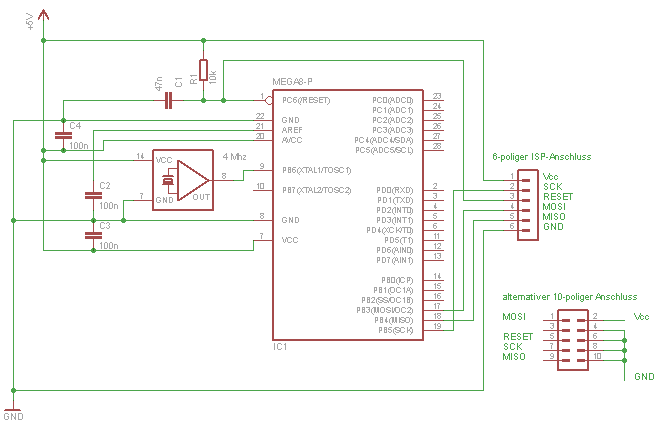
\includegraphics[width=0.7\textwidth]{images/schaltung_minimal.png}
\caption{Grundbeschaltung ATMEGA-Microcontroller}
\label{fig:grundsch}
\end{figure}
 \subsection{ Messen physikalischer Größen}
Meßbereiche -> Spannungsteiler, Op; Schutz -> ZDioden, Schaltplan ...
  
  \subsection{ Kommunikation}
  UART(max232 Chip), CAN(mcp2515+treiber), Schaltplan... 

  
  \subsection{ Reaktionen durch das Meßsystem}
Schaltung von Last durch Relais, Schaltplan...
  
Kenngrößen des Systems:\\
Stromaufnahme: I\textsubscript{default}: 96,7 mA, I\textsubscript{prog}: 86,5 mA, I\textsubscript{Relais 1}: 120,4 mA, I\textsubscript{Relais 2}: 147 mA\\
ADC-Taktung: Datenblatt: 2,08*$10^{-4}$\\
Sende-Taktung: Standard 300ms, Einstellbar durch Poti

\begin{figure}[htb]
\centering
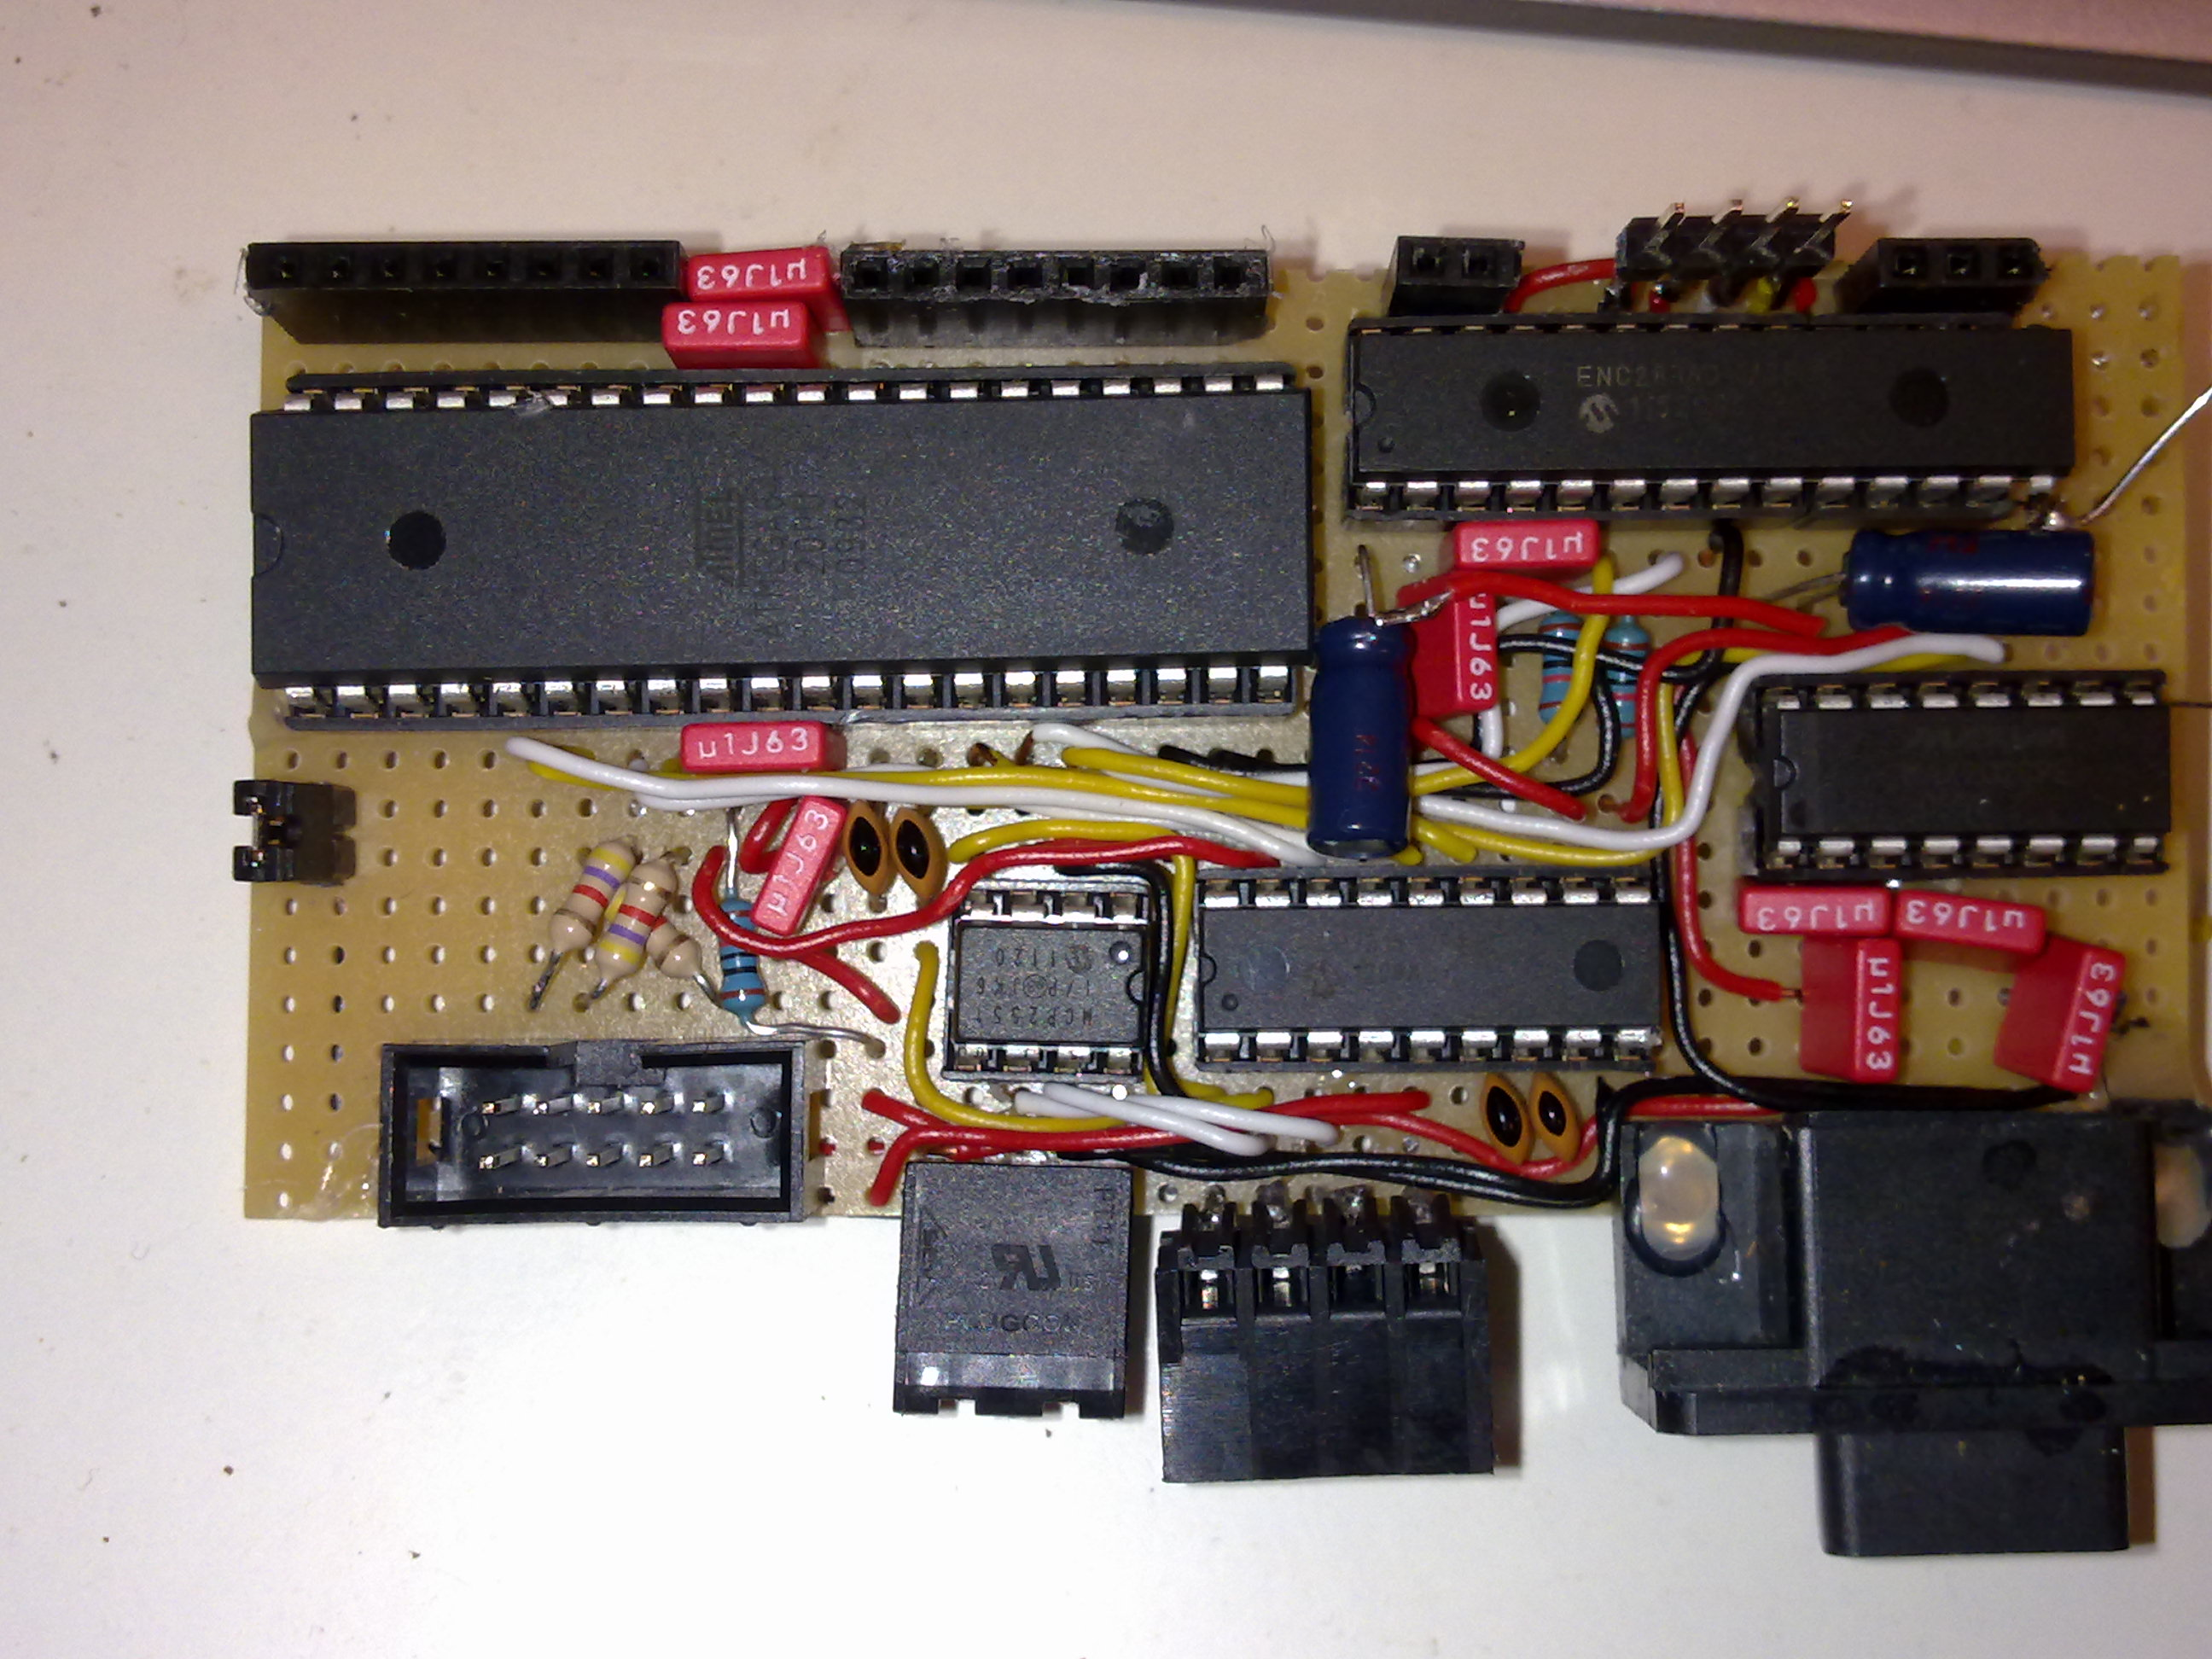
\includegraphics[width=0.6\textwidth]{images/prototyp.jpg}
\caption{Prototyp des Kommunikations- und Kontrollteils}
\label{fig:prototyp}
\end{figure}


\section{Software}

  \subsection{Microcontroller}
    Die Übertragung der in der Programmiersprache C geschriebenen und durch den gcc-Compiler compilierten Datei vom PC auf den Microcontroller erfolgt hardwareseitig mittels eines Adapters\footnote{USBasp - USB programmer for Atmel AVR controllers http://www.fischl.de/usbasp/}, softwareseitig mittels des
  Tools avrdude. Die erste grundlegende Programmierung des Microcontrollers erfolgte durch die Implementierung einer getakteten Ansteuerung einer LED in C Code und anschließender Übertragung
  des Codes auf den Microcontroller mittels des usbasp Adapters. Die Implementierung der verschiedenen Funktionen zum Senden und ....\cite{8}.

  \begin{figure}[htb]
\centering
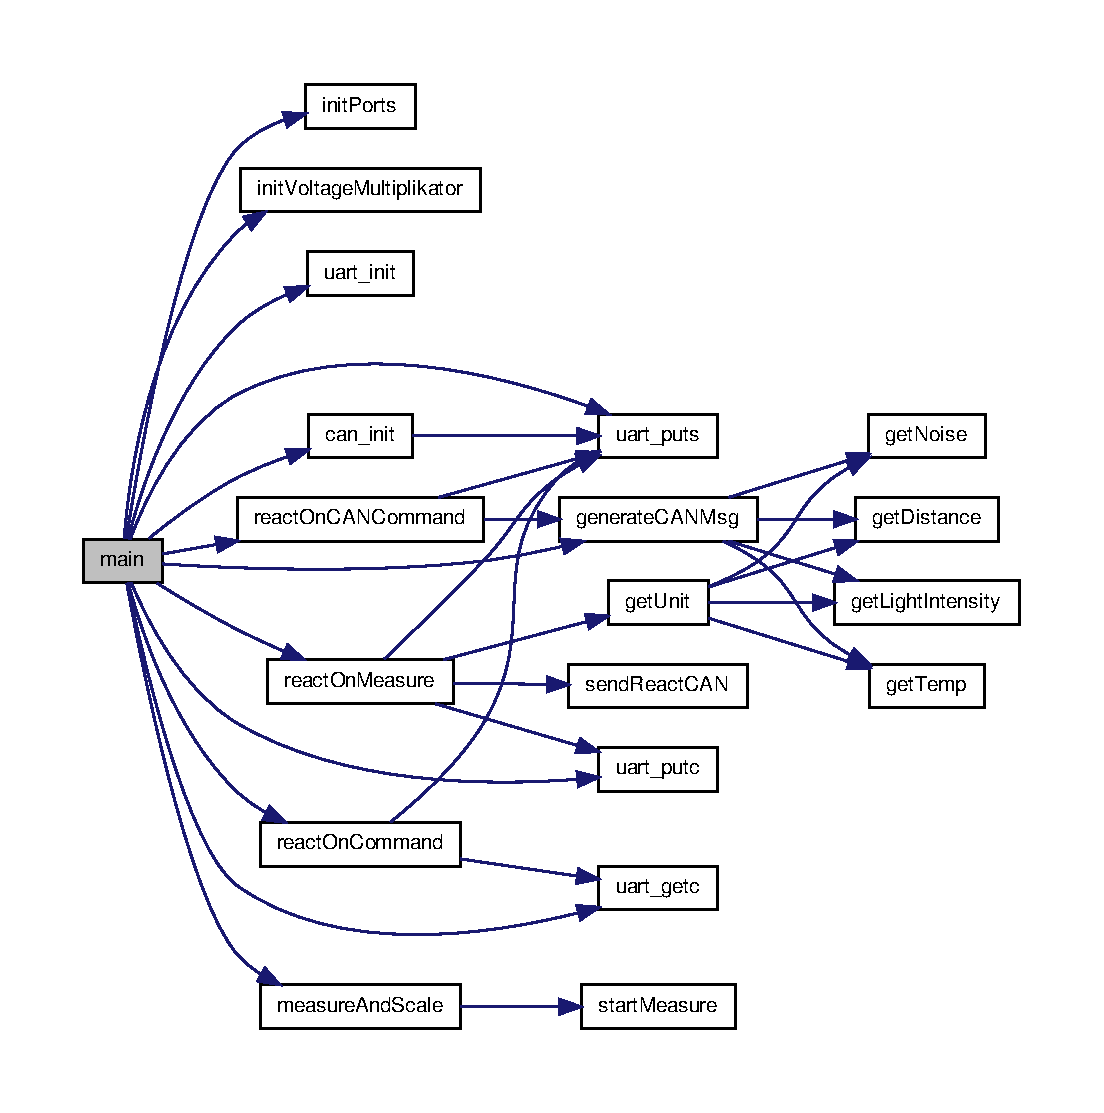
\includegraphics{images/main.pdf}
\caption{Callgraph main-Methode}
\label{fig:prototyp}
\end{figure}
 
  
  \subsection{Robotersystem}
  
  Beschreibung d. software \\
  
\begin{figure}[htb]
\centering
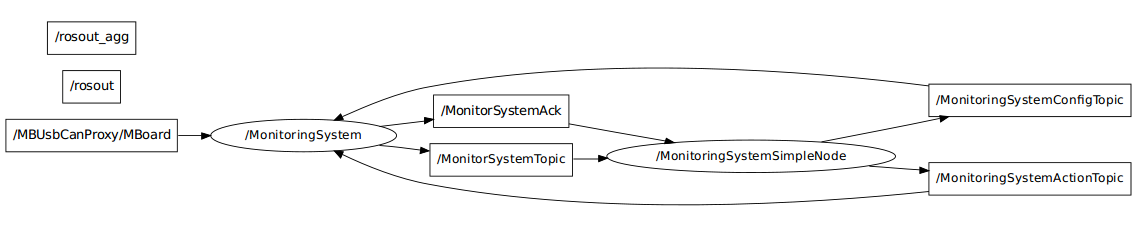
\includegraphics[width=1.0\textwidth]{images/ros.png}
\caption{Aufbau des Robotersystems}
\label{fig:prototyp}
\end{figure}
 






\chapter{Evaluierung}

\label{cha:Evaluierung}
Im folgenden Kapitel wird die Evaluierung des Projektes dargestellt, die Tests der Hard-und Software erfolgen mittels verschiedener Versuchsaufbauten. 
\section{Messen}
Die Evaluierung der Funktionalität Messen
erfolgt mittels eines Multimeter zur Ermittlung des tatsächlichen Spannungswertes, das Netzteil des Fachgebietes dient zur 
Versorgung des Versuchsaufbaues. Abbildung~\ref{fig:aufbau} zeigt den Versuchsaufbau, Abbildungen~\ref{fig:5v},~\ref{fig:26v},~\ref{fig:mv}  die erfassten Spannungswerte des Meßgerätes und des Meßsystemes.


\begin{figure}[htb]
\centering
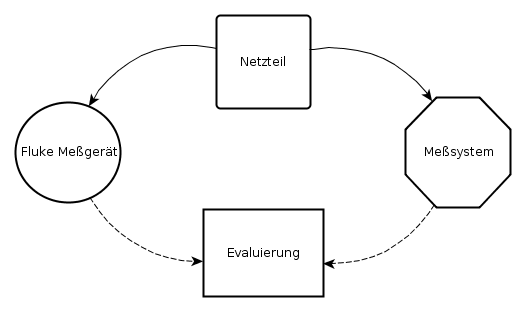
\includegraphics[width=0.6\textwidth]{images/evalSpannung.png}
\caption{Aufbau zur Evaluierung der Funktionalität Messen}
\label{fig:aufbau}
\end{figure}

\begin{figure}[htb]
\centering
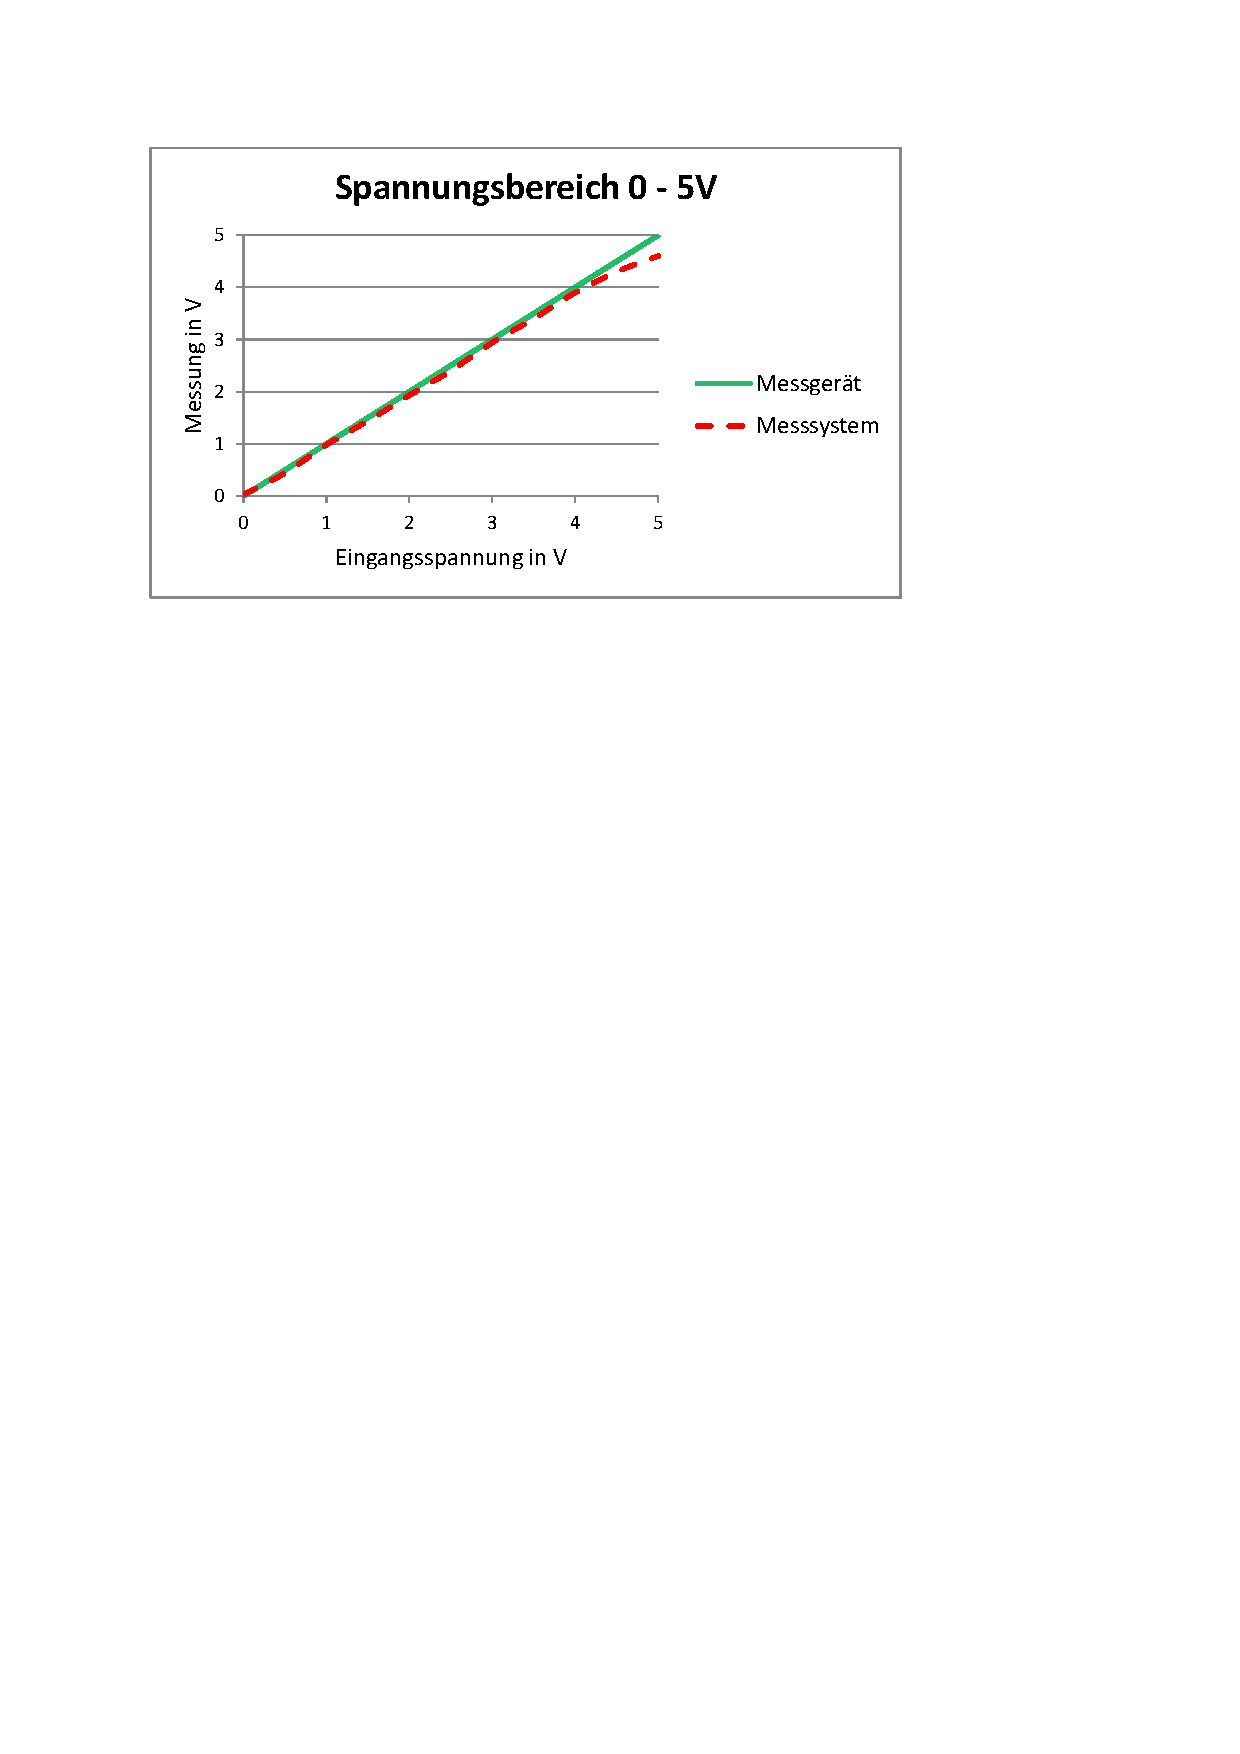
\includegraphics[width=0.7\textwidth]{images/5vpdf.pdf}
\caption{Messungen 0-5V}
\label{fig:5v}
\end{figure}

\begin{figure}[htb]
\centering
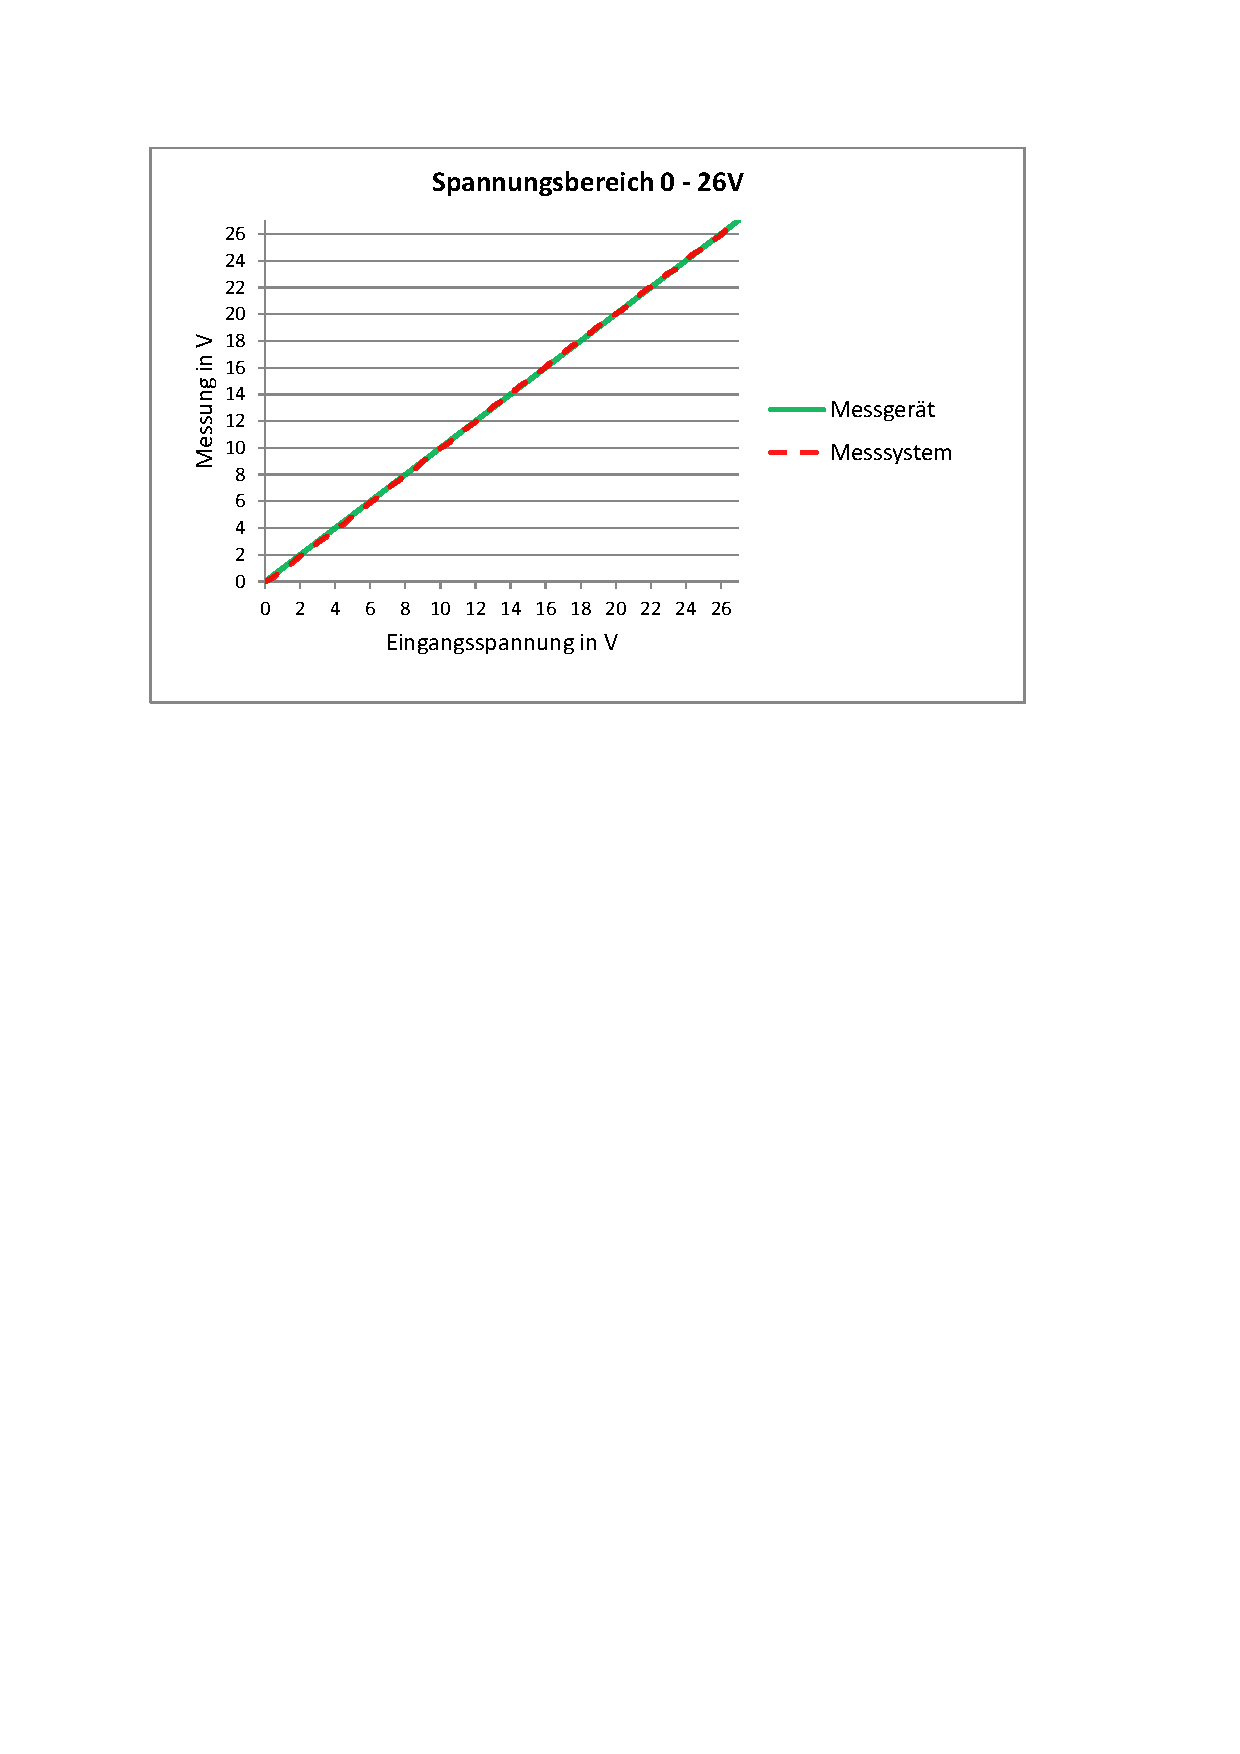
\includegraphics[width=0.7\textwidth]{images/26Vpdf.pdf}
\caption{Messungen 0-26V}
\label{fig:26v}
\end{figure}

\begin{figure}[htb]
\centering
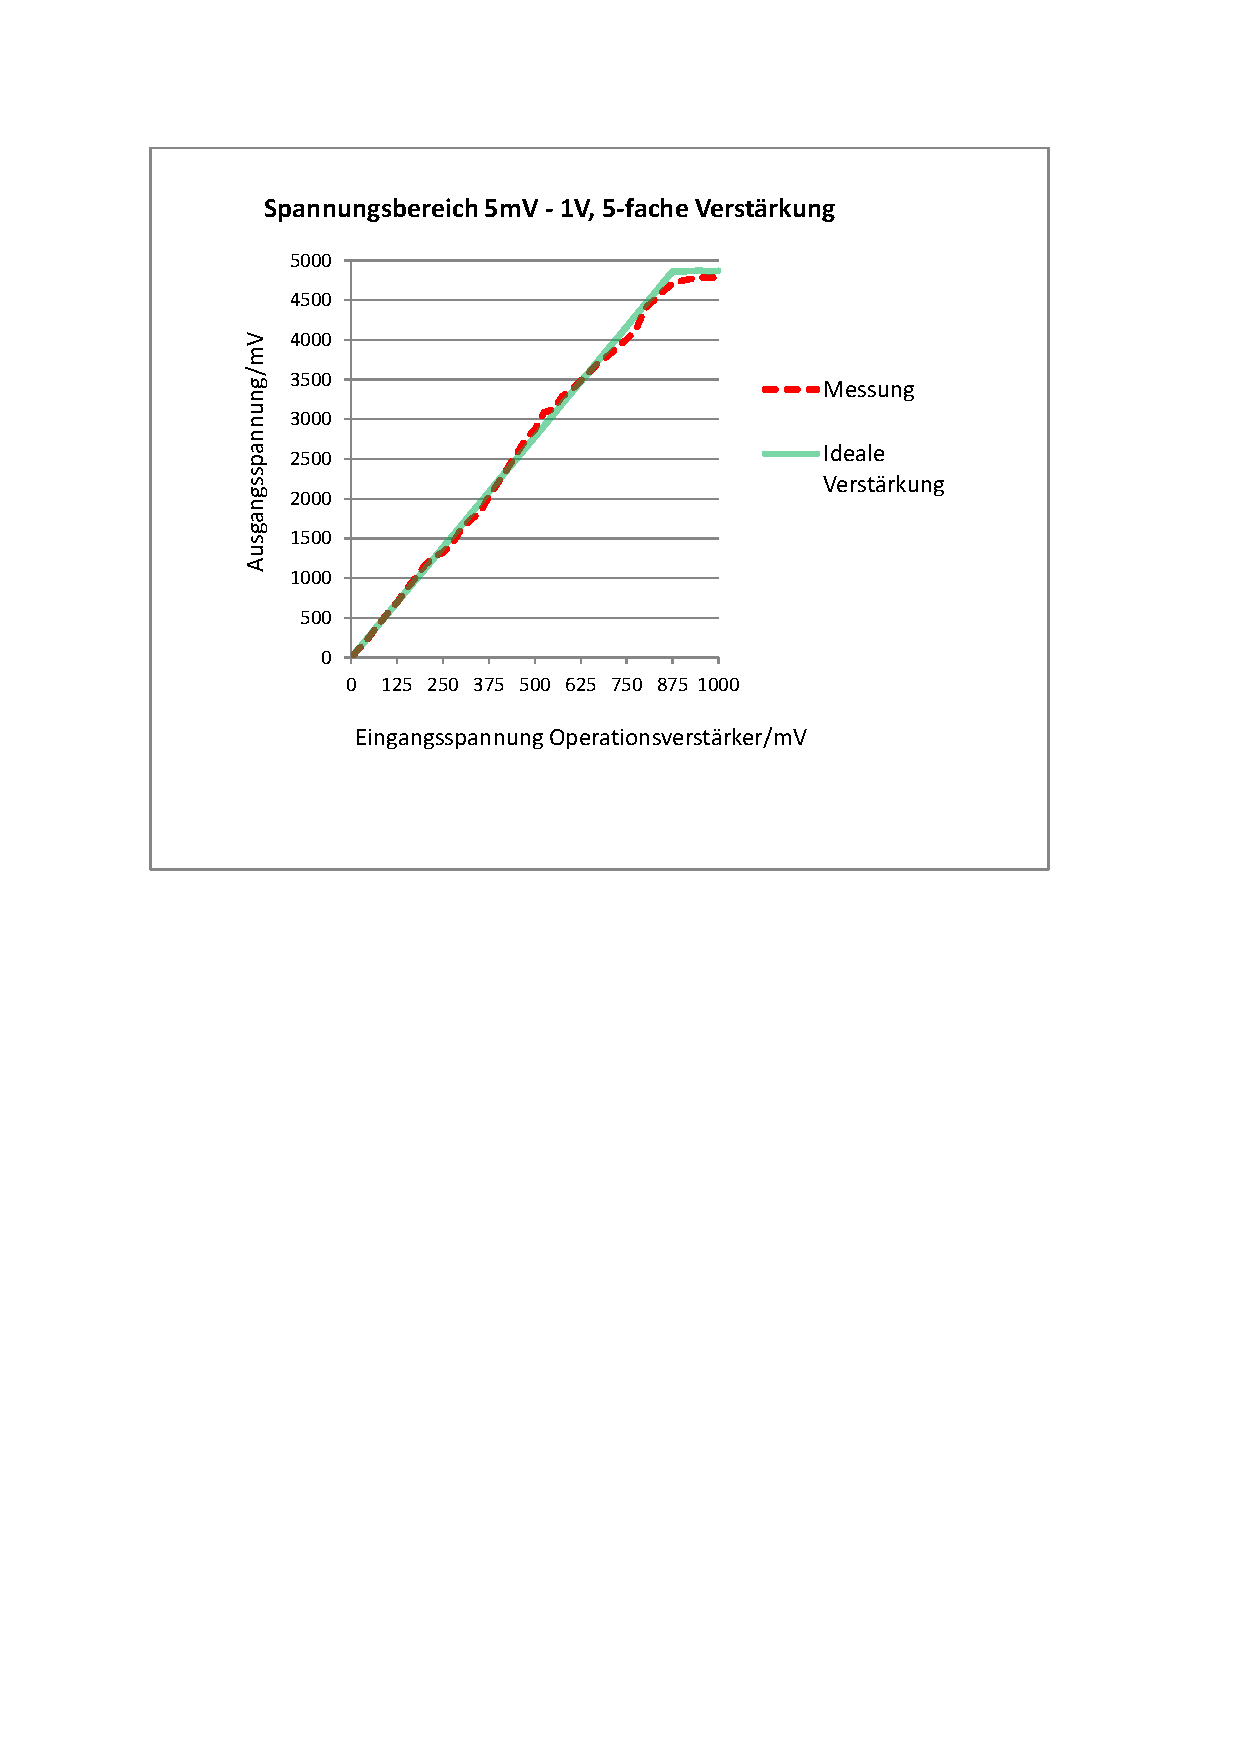
\includegraphics[width=0.7\textwidth]{images/mVpdf.pdf}
\caption{Messungen 0-5V}
\label{fig:mv}
\end{figure}

\section{Kommunikation}
.....\\
\section{Reaktion}
...\

%\begin{tabular}{lllllll}
%Spannungswert & Messung  0 & Messung 2 & Messung 3 & Messung 4 & Messung 5 & Messung 6\\
%0 V & 0 & 0 & 0 & 0 & 0 & 0\\
%1,3 V & 0 & 0 & 0 & 0 & 0 & 0\\
%2,5 V & 0 & 0 & 0 & 0 & 0 & 0\\
%3,5 V & 0 & 0 & 0 & 0 & 0 & 0\\
%4,9 V & 0 & 0 & 0 & 0 & 0 & 0
%\end{tabular}



\chapter{Zusammenfassung}
\label{cha:Zusammenfassung}
Zusammenfassung .... es funktioniert :-D

%\chapter{Abbildungsverzeichnis}
%\label{cha:Abbildungsverzeichnis}

%\chapter{Literaturverzeichnis}
 
  
 \bibliography{literatur}{}
 \bibliographystyle{plain}

%\bibliography{bibtex_database}

\end{document}
